% This file was created by tikzplotlib v0.9.1.
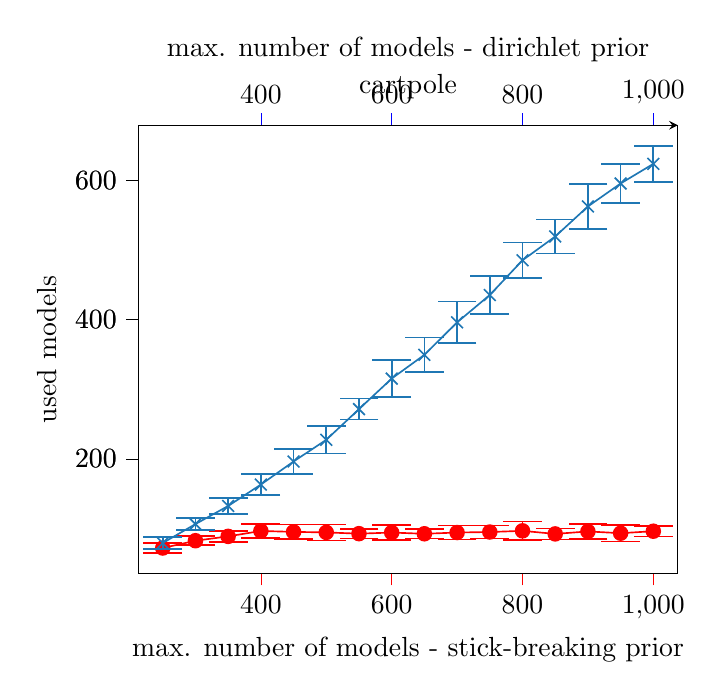
\begin{tikzpicture}

\definecolor{color0}{rgb}{0.12156862745098,0.466666666666667,0.705882352941177}

\begin{axis}[
tick align=outside,
tick pos=left,
title={cartpole},
x grid style={white!69.0196078431373!black},
xlabel={max. number of models - stick-breaking prior},
xmin=212.5, xmax=1037.5,
xtick style={color=red},
y grid style={white!69.0196078431373!black},
ylabel={used models},
ymin=35.2334307476987, ymax=678.878100769765,
ytick style={color=black}
]
\path [draw=red, semithick]
(axis cs:250,64.4900066577926)
--(axis cs:250,79.5099933422074);

\path [draw=red, semithick]
(axis cs:300,75.8823034322576)
--(axis cs:300,89.0776965677424);

\path [draw=red, semithick]
(axis cs:350,80.9610309963243)
--(axis cs:350,96.4789690036757);

\path [draw=red, semithick]
(axis cs:400,86.7511974015298)
--(axis cs:400,106.20880259847);

\path [draw=red, semithick]
(axis cs:450,84.6769470095778)
--(axis cs:450,105.643052990422);

\path [draw=red, semithick]
(axis cs:500,82.914356787711)
--(axis cs:500,105.885643212289);

\path [draw=red, semithick]
(axis cs:550,85.4445824720007)
--(axis cs:550,99.7554175279993);

\path [draw=red, semithick]
(axis cs:600,83.7042865892785)
--(axis cs:600,104.695713410722);

\path [draw=red, semithick]
(axis cs:650,85.8364857840692)
--(axis cs:650,99.0435142159308);

\path [draw=red, semithick]
(axis cs:700,84.2789558780216)
--(axis cs:700,104.201044121978);

\path [draw=red, semithick]
(axis cs:750,85.564341428085)
--(axis cs:750,104.355658571915);

\path [draw=red, semithick]
(axis cs:800,83.4010272301813)
--(axis cs:800,109.878972769819);

\path [draw=red, semithick]
(axis cs:850,84.3341540617085)
--(axis cs:850,100.145845938291);

\path [draw=red, semithick]
(axis cs:900,84.6860448084402)
--(axis cs:900,106.91395519156);

\path [draw=red, semithick]
(axis cs:950,81.5342944017824)
--(axis cs:950,105.025705598218);

\path [draw=red, semithick]
(axis cs:1000,88.6403208624968)
--(axis cs:1000,103.599679137503);

\addplot [semithick, red, mark=-, mark size=7, mark options={solid}, only marks]
table {%
250 64.4900066577926
300 75.8823034322576
350 80.9610309963243
400 86.7511974015298
450 84.6769470095778
500 82.914356787711
550 85.4445824720007
600 83.7042865892785
650 85.8364857840692
700 84.2789558780216
750 85.564341428085
800 83.4010272301813
850 84.3341540617085
900 84.6860448084402
950 81.5342944017824
1000 88.6403208624968
};
\addplot [semithick, red, mark=-, mark size=7, mark options={solid}, only marks]
table {%
250 79.5099933422074
300 89.0776965677424
350 96.4789690036757
400 106.20880259847
450 105.643052990422
500 105.885643212289
550 99.7554175279993
600 104.695713410722
650 99.0435142159308
700 104.201044121978
750 104.355658571915
800 109.878972769819
850 100.145845938291
900 106.91395519156
950 105.025705598218
1000 103.599679137503
};
\addplot [semithick, red, mark=*, mark size=2.5, mark options={solid}]
table {%
250 72
300 82.48
350 88.72
400 96.48
450 95.16
500 94.4
550 92.6
600 94.2
650 92.44
700 94.24
750 94.96
800 96.64
850 92.24
900 95.8
950 93.28
1000 96.12
};
\end{axis}

\begin{axis}[
axis x line=top,
tick align=outside,
x grid style={white!69.0196078431373!black},
xlabel={max. number of models - dirichlet prior},
xmin=212.5, xmax=1037.5,
xtick pos=right,
xtick style={color=blue},
y grid style={white!69.0196078431373!black},
ymin=35.2334307476987, ymax=678.878100769765,
ytick pos=left,
ytick style={color=black}
]
\path [draw=color0, semithick]
(axis cs:250,70.9924306610978)
--(axis cs:250,87.4875693389022);

\path [draw=color0, semithick]
(axis cs:300,97.7072316568626)
--(axis cs:300,115.012768343137);

\path [draw=color0, semithick]
(axis cs:350,121.199784948309)
--(axis cs:350,143.520215051691);

\path [draw=color0, semithick]
(axis cs:400,147.993794380296)
--(axis cs:400,178.166205619704);

\path [draw=color0, semithick]
(axis cs:450,178.356233581444)
--(axis cs:450,214.043766418556);

\path [draw=color0, semithick]
(axis cs:500,207.856400332246)
--(axis cs:500,246.863599667754);

\path [draw=color0, semithick]
(axis cs:550,256.302980426588)
--(axis cs:550,286.497019573412);

\path [draw=color0, semithick]
(axis cs:600,288.690001883239)
--(axis cs:600,341.789998116761);

\path [draw=color0, semithick]
(axis cs:650,324.663635895136)
--(axis cs:650,374.056364104864);

\path [draw=color0, semithick]
(axis cs:700,365.922773461535)
--(axis cs:700,425.917226538465);

\path [draw=color0, semithick]
(axis cs:750,408.2163417107)
--(axis cs:750,462.3436582893);

\path [draw=color0, semithick]
(axis cs:800,459.36320393206)
--(axis cs:800,510.79679606794);

\path [draw=color0, semithick]
(axis cs:850,494.801639399337)
--(axis cs:850,543.598360600663);

\path [draw=color0, semithick]
(axis cs:900,529.714167187832)
--(axis cs:900,595.005832812168);

\path [draw=color0, semithick]
(axis cs:950,567.336118925353)
--(axis cs:950,623.303881074647);

\path [draw=color0, semithick]
(axis cs:1000,597.418475140329)
--(axis cs:1000,649.621524859671);

\addplot [semithick, color0, mark=-, mark size=7, mark options={solid}, only marks]
table {%
250 70.9924306610978
300 97.7072316568626
350 121.199784948309
400 147.993794380296
450 178.356233581444
500 207.856400332246
550 256.302980426588
600 288.690001883239
650 324.663635895136
700 365.922773461535
750 408.2163417107
800 459.36320393206
850 494.801639399337
900 529.714167187832
950 567.336118925353
1000 597.418475140329
};
\addplot [semithick, color0, mark=-, mark size=7, mark options={solid}, only marks]
table {%
250 87.4875693389022
300 115.012768343137
350 143.520215051691
400 178.166205619704
450 214.043766418556
500 246.863599667754
550 286.497019573412
600 341.789998116761
650 374.056364104864
700 425.917226538465
750 462.3436582893
800 510.79679606794
850 543.598360600663
900 595.005832812168
950 623.303881074647
1000 649.621524859671
};
\addplot [semithick, color0, mark=x, mark size=3, mark options={solid}]
table {%
250 79.24
300 106.36
350 132.36
400 163.08
450 196.2
500 227.36
550 271.4
600 315.24
650 349.36
700 395.92
750 435.28
800 485.08
850 519.2
900 562.36
950 595.32
1000 623.52
};
\end{axis}

\end{tikzpicture}
